
\section{Driver}
\label{sec:driver}

The part that does all the acting in this world is the drivers. A
driver looks at the world (\ref{sec:sight}), assesses the situation
and reacts accordingly (\ref{sec:animus}), decides about which
way to go (\ref{sec:driverJunctions}) and eventually steers the
vehicle (\ref{sec:driverInfluence}). Drivers have a character
(\ref{sec:character}) and physical conditions (\ref{sec:physics}). They
can also take drugs (\ref{sec:drugs}). \\

\subsection{Animus}
\label{sec:animus}

The Animus is the brain of the driver. Here all way points 
(\ref{sec:wayPointSystem}) are processed and decisions are made. \\

\noindent The Animus only knows the current speed limit on the lane 
(before the driver has seen any speed limit signs this is some global
default value). It then assesses the situation in following order:

\begin{itemize}
\item Look at the world and collect way points (assessment)
\item 
\end{itemize}

\subsubsection{Assessment and decision making}

\begin{figure}[H]
\begin{center}
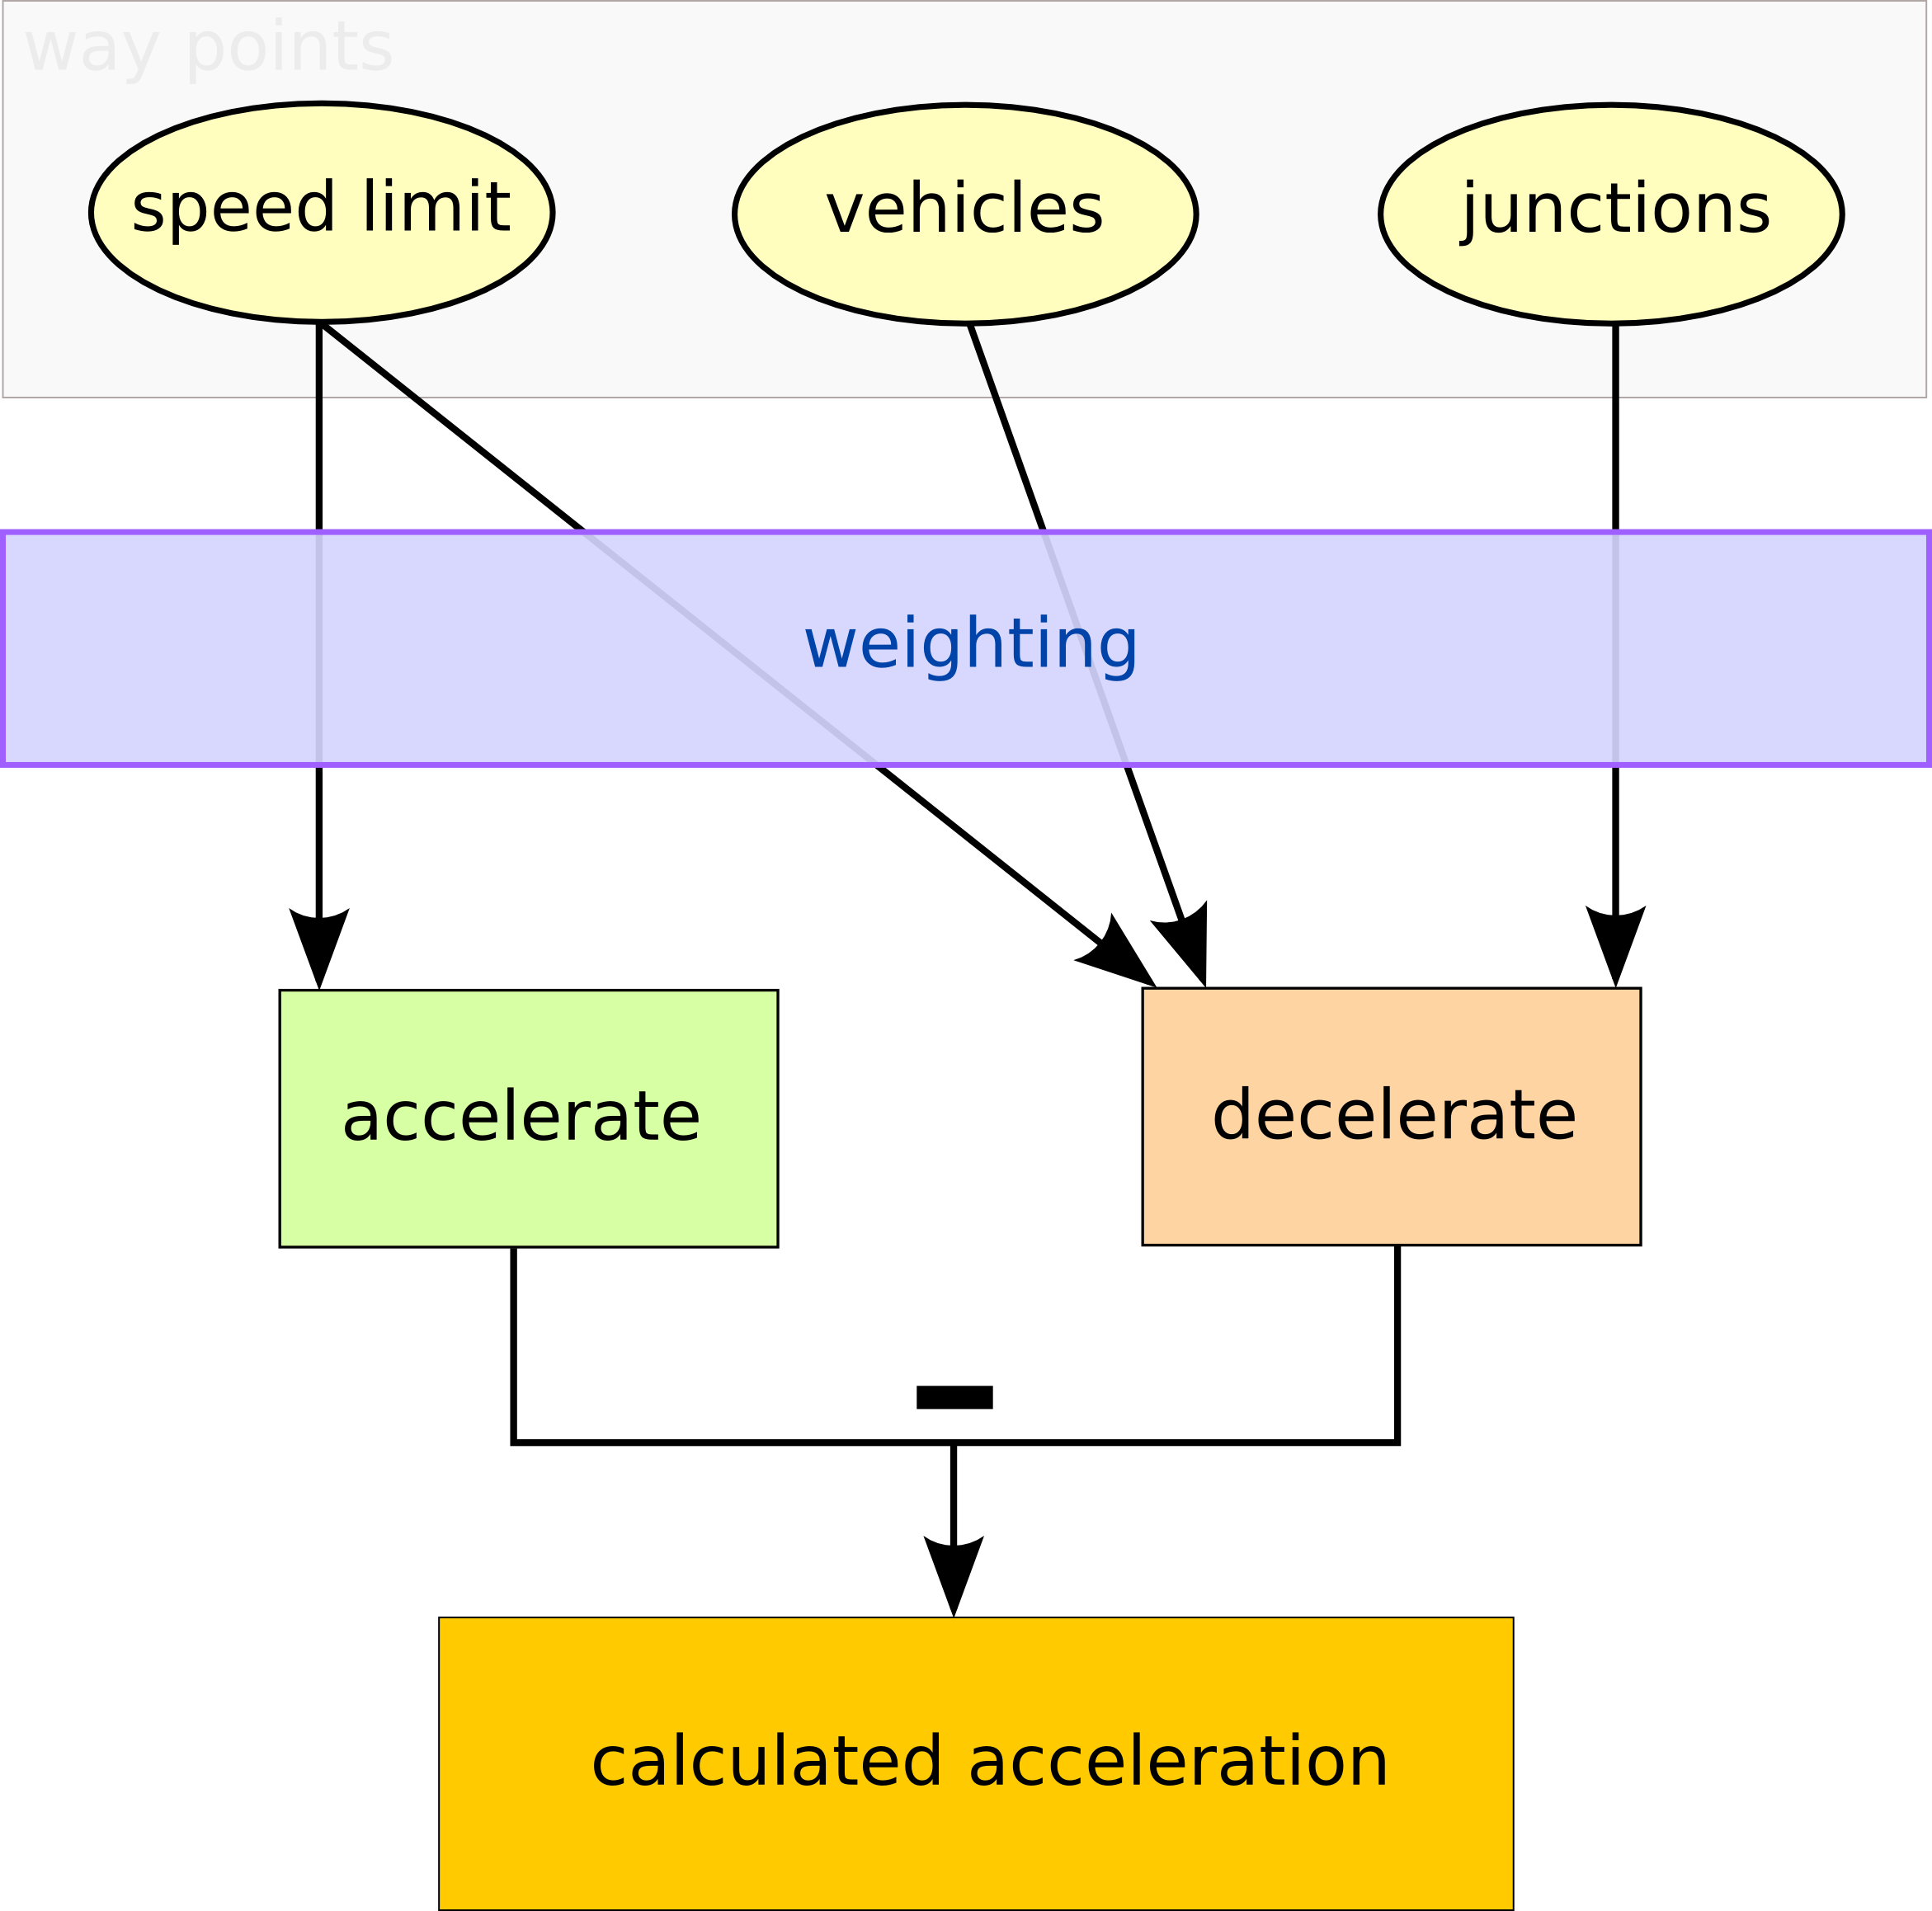
\includegraphics[width=\textwidth]{images/animus.png}
\end{center}
\caption{The assessment process}
\label{fig:animus}
\end{figure}

\subsubsection{The estimation of another vehicle's speed}

To know whether another vehicle is approaching (because it moves 
more slowly) or not, we could have just implemented a method on the
way point that returns the speed of it's vehicle to the driver that
is assessing. But we wanted it more realistic, the drivers should have
to estimate the speed of the other traffic participants. They can
therefore only retrieve the fuzzy distance (\ref{par:movingWPDistance})
to the other way points. A driver then has to remember the distance
of the nearest vehicle, until the next assessment cycle. It can then
compare the remembered distance with the new one and knows, whether the
vehicle is approaching or not and how fast.

\subsubsection{Following another vehicle}

When a driver sees another vehicle in front of him, it retrieves the distance
of this v

% mention how the speed is calculated
% brakeway
% 

\subsubsection{Decisions in junctions}

\subsection{Physics}
\label{sec:physics}

The physics objects define the physical conditions of the driver. Every
driver has one of these objects. They provide following properties:

\begin{itemize}
\item \textbf{The sight} How far the driver can see
\item \textbf{The field of view (angle)} The opening of the driver view
\item \textbf{Update interval} The interval of the assessment cycles
\item \textbf{Drugs}
\end{itemize}

\subsubsection{Drugs}
\label{sec:drugs}

Drugs are objects than can influence the properties mentioned above in the
physics section. They are merely just implemented and prepared but not 
in use yet.

\subsection{Character}
\label{sec:character}

\subsection{Sight}
\label{sec:sight}

At this point of process the driver only sees things ahead of him on the
lane. There are no mirrors, and it is not possible to look behind, hence
he is not able to reverse.\\

\noindent What the driver can see is limited to a field of view formed as 
a ''Pacman``. We implemented that as the \emph{driver view}, more on that in 
section \ref{sec:driverView}.

\subsection{Junctions}
\label{sec:driverJunctions}

When a driver approaches a junction, he receives the according way point
from the way point system. He then makes a decision in which direction he
wants to drive on. Since we don't have any path finding and the cars are
just driving around, this decision is randomly taken. Once decided, a
driver event is created and processed immediately which then triggers
the junction routine of the vehicle (\ref{sec:laneChanges}).

